
\subsection{Λογική και Design Patterns}

\subsubsection{Γραμμική Λογική}

Η λογική είναι από τις σημαντικότερες αρχές της Rust καθώς
αποτυπώνει με αυστηρό μαθηματικό τρόπο τους υποκείμενους
μηχανισμούς του μεταγλωττιστή. Μάλιστα έχουμε ήδη αναφέρει ότι
όλες οι γλώσσες συμπίπτουν στη επιστήμη της λογικής με τον έναν
ή τον άλλον τρόπο, σε καμία περίπτωση όμως δεν είναι απαραίτητη
για την κατανόηση τους. Γιατί λοιπόν είναι εξαίρεση η Rust?
Η λέξη κλειδί είναι η αυστηρότητα της γλώσσας και η απαίτηση του
μεταγλωττιστή ένα πρόγραμμα να είναι σωστό με βάσει προορισμένους
κανόνες. Το σύστημα λογικής που χρησιμοποιείτε για να εκφράσει την
εγκυρότητα ενός προγράμματος είναι ένα υποσύνολο της γραμμικής λογικής
(Linear Logic).

Στις συνηθισμένες λογικές/γλώσσες προγραμματισμού χρησιμοποιούμε $\phi \vdash \psi$
εννοώντας ότι εφόσον ξέρουμε την εγκυρότητα του $\phi$ μπορούμε να συμπεράνουμε
την εγκυρότητα του $\psi$. Η σχέση αυτή διατηρείτε για πάντα, ανεξαρτήτως της
κατάστασης, μόλις αποδείξουμε ότι $\psi$ είναι αληθές επειδή το $\phi$ είναι
αληθές δεν μπορούμε ξαφνικά να αλλάξουμε γνώμη, $\phi \rightarrow true$ για
πάντα αλλιώς αλλάζει και το αποτέλεσμα του $\psi$. Αυτό έχει ως αποτέλεσμα
ορισμένα συμπεράσματα να είναι πολύ πιθανά, για παράδειγμα έστω $\Alpha \rightarrow \Beta,
\Alpha \rightarrow \Gamma$, τότε ένα ενδεχόμενο συμπέρασμα μπορεί να είναι $\Alpha \vdash \Beta \land \Gamma$.
Το παραπάνω παράδειγμα αν και συμβατό με την πραγματικότητα δεν μοντελοποιεί πλήρως
ένα \textbf{σωστό} πρόγραμμα. Αν το $\Alpha$ ήταν πρόσβαση σε έναν πόρο όπως ένα αρχείο
δεν μπορούμε να το επαναχρησιμοποιήσουμε και για το $\Beta$  και για το $\Gamma$, τι γίνεται
αν ένα από τα δύο απενεργοποιήσει τον πόρο ή στο παράδειγμα μας κλείσει το αρχείο? Χρειαζόμαστε
λοιπόν έναν τρόπο να ελέγχουμε για αυτές τις περιπτώσεις.

Η γραμμική λογική προσθέτει την έννοια της κατανάλωσης. Με $\Alpha \multimap \Beta$
εννοούμε ότι για \textbf{ένα} $\Alpha$ παράγετε \textbf{ένα} $\Beta$. Προσθέτοντας
επίσης έναν εναλλακτικό τελεστή για το "γραμμικό λογικό και" $\otimes$ ισχύει ότι:

\begin{center}
    \begin{math}
    \Alpha \multimap \Beta,\Alpha \multimap \Gamma, \Alpha \nvdash \Beta \otimes \Gamma
    \end{math}
\end{center}

Το $\Alpha$ καταναλώνετε από την πιο αριστερή οντότητα, κατά σύμβαση, το $\Beta$.
Με τον ίδιο συνειρμό ισχύει  $\Alpha \multimap \Beta,\Alpha \multimap \Gamma, \Alpha,\Alpha \vdash \Beta \otimes \Gamma$
καθώς τώρα έχουμε δύο οντότητες του $\Alpha$ η κάθε μια θα καταναλωθεί από το $\Beta$ και $\Gamma$ αντίστοιχα. Το γεγονός
ότι ο μεταγλωττιστής καταλαβαίνει την γραμμική λογική δεν σημαίνει ότι την αντικαθιστά οποιαδήποτε άλλη πλήρως.

Πολλές φορές είναι απαραίτητο να παραχθούν $v\in\mathbb{N} $ αναφορές (references) αμετάβλητης μορφής, δηλαδή ισχύει:

\begin{equation}
\alpha:T \rightarrow \beta: \&T
\end{equation}

Όμως δεν μπορούμε να έχουμε παραπάνω από μια αναφορά αν είναι μεταβλητή, σε αυτήν την περίπτωση καταναλώνετε:

\begin{equation}
\alpha:T \multimap \beta: \& mut T
\end{equation}

Το ίδιο ισχύει για οποιαδήποτε μη-αντιγράψιμη τιμή:

\begin{equation}
\alpha:T \multimap \beta: T
\end{equation}

Ορισμένοι τύποι όμως είναι υπερβολικά πολύ εύκολο να αντιγραφθούν χρησιμοποιόντας κάποιου είδους
\verb|memcpy|, για παράδειγμα \verb|u8|. Αυτοί οι τύπου είναι αντιγράψιμοι.

\begin{equation}
\alpha:T \textup{ is Copy } \rightarrow \beta:T
\end{equation}

Η έννοια της κατανάλωσης της γραμμικής λογικής είναι ίδια ακριβώς με την έννοια
της ιδιοκτησίας (ownership) της Rust. Παρακάτω είναι μερικά ακόμη παραδείγματα.

\begin{lstlisting}[language=Rust]
struct T;

fn reference_infinite_times(a: T) -> T {
    let b = &a;
    let c = &a;
    let d = &a;
    // let e = &mut a; Error, cant consume variable
    // that is referenced in its lifetime
    return a;
}

fn mutate_reference(mut a: &mut T) -> &mut T {
    let b = a;
    // return a; Error, use of consumed variable 'a'
    return b;
}

fn consume_and_return(a: T) -> T {
    let b = a;
    // let c = a; Error, use of consumed variable 'a'
    return b;
}

fn can_copy(mut a: u8) -> u8 {
    let b = a;
    let c = a;
    let d = &mut a;
    let e = &a;

    return a;
}

fn main() {
    let v0: T = T;

    let v1 = reference_infinite_times(v0);
    //infinite_references(var0); Error,
    //use of consumed variable 'v0'

    let mut v2 = consume_and_return(v1);
    //infinite_references(var1); Error,
    //use of consumed variable 'v1'

    let v3 = mutate_reference(&mut v2);
    //v2 is consumed, mutated and returned as v3

    let v = can_copy(42);
}
\end{lstlisting}

\subsubsection{Builder Pattern}

Ίσως το πιο διαδεδομένο pattern που η λογική της Rust βοηθάει να μοντελοποιήσει
είναι το Builder Pattern (πρότυπο κατασκευαστή). Επιτρέπει την κατασκευή
σύνθετων αντικειμένων βήμα προς βήμα χρησιμοποιώντας την γραμμική λογική
για να μπορέσουμε να ρυθμίσουμε το αντικείμενο ανάλογα με τις ανάγκες μας.

Όταν ένα struct διαθέτει πολλές προαιρετικές παραμέτρους, η χρήση μιας
απλής συνάρτησης αρχικοποίησης τύπου \verb|new| μπορεί να οδηγήσει σε δύσκολη
συντήρηση και δυσανάγνωστο κώδικα. Χαρακτηριστικό παράδειγμα είναι η
δημιουργία μιας δομής Car με πολλά χαρακτηριστικά:

\begin{lstlisting}[language=Rust]
struct Car {
    brand: String,
    model: String,
    year: u16,
    color: String,
    automatic: bool,
}
\end{lstlisting}

Ένας κλασικός τρόπος για την αρχικοποίηση ενός αντικειμένου είναι η χρήση μιας συνάρτησης:

\begin{lstlisting}[language=Rust]
impl Car {
    fn new(brand: &str, model: &str, year: u16, color: &str, automatic: bool) -> Self {
        Car {
            brand: brand.to_string(),
            model: model.to_string(),
            year,
            color: color.to_string(),
            automatic,
        }
    }
}

let car = Car::new("Toyota", "Corolla", 2022, "Blue", true);
\end{lstlisting}

Αυτός ο τρόπος δημιουργίας έχει τρία βασικά προβλήματα:

\begin{itemize}
\item Η σειρά των ορισμάτων είναι αυστηρή, το οποίο για μεγάλες βιβλιοθήκες ή σύνθετα
  drivers μπορεί να προκαλέσει σύγχυση στον χρήστη.
\item Η ανάγνωση του κώδικα είναι δυσανάγνωστη, ιδιαίτερα όταν υπάρχουν πολλές παράμετροι.
\item Το αντικείμενο δεν είναι ρυθμιζόμενο ενώ θα μπορούσε να είναι. Έστω δηλαδή ότι όλα
  τα αυτοκίνητα είναι manual, του 2020 και άσπρα εκτός αν ρυθμιστούν αλλιώς.
\end{itemize}

Το Builder Pattern αντιμετωπίζει αυτά τα προβλήματα, επιτρέποντας τη
σταδιακή διαμόρφωση ενός αντικειμένου μέσω αλυσίδωσης μεθόδων (method
chaining). Αυτές οι μέθοδοι ρύθμισης καταναλώνουν τον Builder και επιστρέφουν τον
μεταλλαγμένο Builder με τα καινούργια πλέον πεδία επιτρέποντας να συνεχίσει η αλυσίδα
ή να καλεστεί η τελική μέθοδος build που θα καταναλώσει τον Builder για μια τελευταία
φορά και θα δημιουργήσει ένα αντικείμενο Car.

Παρακάτω δίνεται μια υλοποίηση του προτύπου για το struct Car:

\begin{lstlisting}[language=Rust]
struct Car {
    brand: String,
    model: String,
    year: u16,
    color: String,
    automatic: bool,
}

struct CarBuilder {
    brand: String,
    model: String,
    year: Option<u16>,
    color: Option<String>,
    automatic: Option<bool>,
}

impl CarBuilder {
    fn new(brand: &str, model: &str) -> Self {
        Self {
            brand: brand.to_string(),
            model: model.to_string(),
            year: None,
            color: None,
            automatic: None,
        }
    }

    fn year(mut self, year: u16) -> Self {
        self.year = Some(year);
        self
    }

    fn color(mut self, color: &str) -> Self {
        self.color = Some(color.to_string());
        self
    }

    fn automatic(mut self, automatic: bool) -> Self {
        self.automatic = Some(automatic);
        self
    }

    fn build(self) -> Car {
        Car {
            brand: self.brand,
            model: self.model,
            year: self.year.unwrap_or(2020), // Default value 
            color: self.color.unwrap_or_else(|| "White".to_string()), // Default value
            automatic: self.automatic.unwrap_or(false), // Default value
        }
    }
}

fn main() {
    let car = CarBuilder::new("Toyota", "Corolla")
        .year(2023)
        .color("Red")
        .automatic(true)
        .build();

    println!(
        "Car: {} {} - {} ({}) | Automatic: {}",
        car.brand, car.model, car.year, car.color, car.automatic
    );
}
\end{lstlisting}

Προφανώς είναι αρκετά παραπάνω boilerplate αλλά η χρήση για τον end-user της
βιβλιοθήκης είναι υπερβολικά πιο απλοϊκή. 

\subsubsection{Asynchronous Rust}

Το ασύγχρονο (async) μοντέλο της Rust είναι ένα ιδιαίτερα χρήσιμο
εργαλείο, αλλά για να κατανοηθεί πλήρως είναι απαραίτητη μια εισαγωγή
στις έννοιες των generics.

Τα generics στη Rust επιτρέπουν τη συγγραφή γενικευμένου κώδικα που
μπορεί να λειτουργεί με διάφορους τύπους δεδομένων χωρίς ανάγκη για
επανάληψη. Χρησιμοποιώντας generics, μπορούμε να ορίζουμε συναρτήσεις,
δομές (structs), enumerations (enums) και traits, αυξάνοντας την
επαναχρησιμοποίηση του κώδικα και την ασφάλεια τύπων.

\begin{lstlisting}[language=Rust]
fn get_first_element<T>(slice: &[T]) -> Option<&T> {
    slice.get(0)
}

fn main() {
    let numbers = vec![1, 2, 3];
    let first_number = get_first_element(&numbers);
    println!("First number: {:?}", first_number);

    let words = vec!["hello", "world"];
    let first_word = get_first_element(&words);
    println!("First word: {:?}", first_word);
}
\end{lstlisting}

Τα generics της Rust αποτελούν αφαίρεση χωρίς κόστος εκτέλεσης, καθώς ο
μεταγλωττιστής παράγει εξειδικευμένο κώδικα ανάλογα με τους τύπους που
χρησιμοποιούνται κατά την μεταγλώττιση στο ενδιάμεσο στάδιο THIR. Δηλαδή
για το παραπάνω παράδειγμα η συνάρτηση \verb|get_first_element| παράγει
στην πραγματικότητα δύο συναρτήσεις στον τελικό κώδικα μια που έχει παράμετρο
και output \verb|usize| και μια \verb|&str|. 

\begin{figure}[htb!]
  \centering
  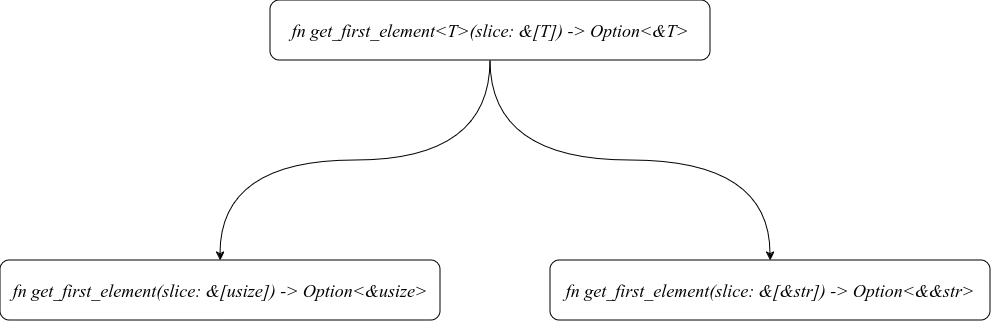
\includegraphics[scale=0.3]{images/rust/rust_generics}
  \caption{Παράδειγμα μεταγλώττισης generics.}
  \label{fig:rust_generic}
\end{figure}

Μπορούμε να περιορίσουμε το σύνολο των πιθανών τιμών ανάλογα με τα
traits (ουσιαστικά interfaces της Java) που υλοποιεί το generic. Για
παράδειγμα, αν θέλουμε μια συνάρτηση να μπορεί να χρησιμοποιεί μόνο
τύπους δεδομένων που υλοποιούν το trait \verb|Display|:

\begin{lstlisting}[language=Rust]
use std::fmt::Display;

fn print_element<T: std::fmt::Display>(element: T) {
    println!("Element: {}", element);
}

fn main() {
    print_element(42);        // i32 implements Display
    print_element("hello");   // &str implements Display
    print_element(vec![1, 2, 3]); // Error: Vec does not implement Display
}
\end{lstlisting}

Το μοντέλο async στην Rust βασίζεται στα Futures τα οποία με την σειρά
τους στηρίζονται πολύ στα generics. Τα Futures είναι traits 
και αντιπροσωπεύουν τιμές που δεν είναι άμεσα διαθέσιμες αλλά θα γίνουν ενδεχωμένος κάποια στιγμή
στο μέλλον. Ο μεταγλωτιστής υλοποιεί τα Futures ως state machines τα οποία δεν τρέχουν κατά
την διάρκεια της εκτέλεσης αλλά καταλήγουν ενσωματωμένα στο τελικό binary ως loops και jumps.

Ένα απλό παράδειγμα χρήσης async είναι το κλασσικό HTTP fetch:

\begin{lstlisting}[language=Rust]
async fn fetch_data(url: &str) -> Result<String, reqwest::Error> {
    let response = reqwest::get(url).await?;
    let body = response.text().await?;
    Ok(body)
}

#[tokio::main]
async fn main() {
    match fetch_data("http://example.com").await {
        Ok(body) => println!("Response: {}", body),
        Err(e) => println!("Error: {:?}", e),
    }
}
\end{lstlisting}

Το γεγονός ότι τα \verb|async| σύμβολα είναι compile time οντότητες αφαιρεί
ένα τεράστιο overhead που έρχεται με την υλοποίηση των παραδοσιακών runtimes.

Για να κατανοήσουμε πλήρως αυτόν μηχανισμό πρέπει να εξετάσουμε πώς αποσαφηνίζεται
(desugar) ένα async block. Στο ενδιάμεσο στάδιο HIR οτιδήποτε σύμβολο είναι \verb|async|
μεταφράζεται στην πρωτόγονη μορφή του, δηλαδή ένα Future με μια generic παράμετρο.

Το Future trait φαίνεται κάπως έτσι:

\begin{lstlisting}[language=Rust]
pub trait Future<Output> {
    // Required method
    fn poll(self: Pin<&mut Self>, cx: &mut Context<'_>) -> Poll<Output>;
}
\end{lstlisting}

Κατά συνέπεια η ταυτότητα της συνάρτησης fetch αποσαφηνίζεται από

\begin{lstlisting}[language=Rust] 
async fn fetch_data(url: &str) -> Result<String, reqwest::Error>
\end{lstlisting}

σε

\begin{lstlisting}[language=Rust] 
fn fetch_data<F: Future<Result<String,reqwest::Error>>>(url: &str) -> F
\end{lstlisting}

Παράλληλα το ενσωματωμένο μέρος της συνάρτησης αντικαθιστά τα \verb|await|
με την μέθοδο \verb|poll| 

\begin{lstlisting}[language=Rust] 
fn fetch_data<F: Future<Result<String,reqwest::Error>>>(url: &str) -> F
    let response = reqwest::get(url).poll(someContext);
    let body = response.text().poll(someContext);
    Ok(body)
}
\end{lstlisting}

Προφανώς η υλοποίηση του Future trait και κατά συνέπεια της μεθόδου \verb|poll|
αλλάζει σε κάθε async οικοσύστημα. Η γενική ιδέα όμως είναι ότι η \verb|poll|
επιστρέφει την κατάσταση της συνάρτησης που καλείτε, δηλαδή:

\begin{enumerate}
  \item Αν περιμένει την σειρά της για το επόμενο κάλεσμα (Waiting).
  \item Αν βρίσκεται στην διαδικασία του καλέσματος (Pending).
  \item Αν είναι έτοιμη και έχει τελειώσει το κάλεσμα (Done). 
\end{enumerate}

Τα enums της Rust μοντελοποιούν τις καταστάσεις σχεδόν πάντα,
το παρακάτω παράδειγμα δεν θα κάνει compile για πολλούς λόγους
και μπορεί να θεωρηθεί ψευδοκώδικας.

\begin{lstlisting}[language=Rust]
  enum FetchDataState
  {
    Waiting,
    Pending,
    Done(Result<&str,reqwest::Error>),
  }
 
  enum RespDataState
  {
    Waiting,
    Pending,
    Done(Result<&str,reqwest::Error>),
  }

  struct get
  {
    state: FetchDataState,
    ...,
  }

  struct resp
  {
    state: RespDataState,
    ...,
  }
  
  impl<Output=Result<&str,reqwest::Error>> Future<Output> for get
  {
    fn poll(self: Pin<&mut Self>,cx: &mut Context<'_>) -> Poll<Output>
    {
      loop
      {
        match &mut this.state
        {
          FetchDataState::Waiting => Poll::Pending,
          FetchDataState::Pending => Poll::Pending,
          FetchDataState::Done(res) => Poll::Ready(res),
        }
      }
    }
  }
 
  impl<Output=Result<&str,reqwest::Error>> Future<Output> for resp
  {
    fn poll(self: Pin<&mut Self>,cx: &mut Context<'_>) -> Poll<Output>
    {
      loop
      {
        match &mut this.state
        {
          RespDataState::Waiting => Poll::Pending,
          RespDataState::Pending => Poll::Pending,
          RespDataState::Done(res) => Poll::Ready(res),
        }
      }
    }
  }
\end{lstlisting}

Μια καλή ερώτηση σε αυτό το σημείο είναι πιο το νόημα? Στο παραπάνω παράδειγμα
είναι ξεκάθαρο ότι δεν γίνεται τίποτα παράλληλα απλώς ελέγχουμε αν η συνάρτηση
έχει τελειώσει και πράγματι αυτή είναι η περίπτωση.

Τα Futures δεν είναι τίποτα χωρίς έναν εκτελεστή (Executor) ο οποίος μπορεί να αλλάζει
την συνάρτηση που καλείτε ανάλογα με το Context της. Ένας εκτελεστής αποτελείτε από
έναν Spawner που προσθέτει ή αφαιρεί συναρτήσεις που επιστρέφουν Futures και έναν Waker
που "ξυπνάει" τις συναρτήσεις από τον Spawner για να ελέγξει την κατάσταση τους.

Στην παρακάτω υλοποίηση ψευδοκώδικα ο εκτελεστής είναι απλώς μια δυναμική λίστα και ο
Spawner μια συνάρτηση που προσθέτει Tasks. 

\begin{lstlisting}[language=Rust]
struct Executor {
    queue: VecDeque<Task>,
}

impl Executor {
    fn new() -> Self {
        Executor {
            queue: VecDeque::new(),
        }
    }

    fn spawn(&mut self, task: Task) {
        self.queue.push_back(task);
    }

    fn run(&mut self) {
        while let Some(mut task) = self.queue.pop_front() {
            let waker = task.get_waker();
            let mut context = Context::from_waker(&waker);
            match task.future.as_mut().poll(&mut context) {
                Poll::Pending => self.queue.push_back(task),
                Poll::Ready(_) => {},
            }
        }
    }
}

struct Task {
    future: Pin<Box<dyn Future<Output = ()>>>,
}

impl Task {
    fn get_waker(&self) -> Waker {
      //Wake the task
    }
}

fn main() {
    let mut executor = Executor { queue: VecDeque::new() };

    executor.queue.push_back(Task::new(fetch_data("http://example.com")));

    executor.run();
}
\end{lstlisting}

Για λόγους αισθητικής τις περισσότερες φορές χρησιμοποιούνται macros τα οποία
κρύβουν την πραγματική λειτουργία του executor. Τα macros στην Rust είναι πάρα
πολύ έξυπνα και μπορούν να διαβάσουν πρακτικά όλο το συντακτικό της γλώσσας. Κατά
συνέπεια μια συνάρτηση για παράδειγμα με τον εκτελεστή της embassy φαίνεται έτσι:

\begin{lstlisting}[language=Rust]
#[esp_hal_embassy::main]
async fn main(spawner: Spawner)
{
  //do stuff
  //spawn tasks
  spawner.spawn(task1()).ok();
  spawner.spawn(task2()).ok();
}
\end{lstlisting}

Προφανώς εδώ δεν φαίνεται να ορίζουμε κανέναν εκτελεστή και δεν
υπάρχει καμία λούπα που να τρέχει τα tasks. Για τις περισσότερες
εφαρμογές αυτό είναι ίσως πιο επιθυμητό στην δικιά μας περίπτωση όμως
θέλουμε τα τρέχουμε χρονομετρητές πριν και μετά από κάθε poll που εκτελείται. Ήμαστε
αναγκασμένοι λοιπόν να αποσαφηνίσουμε τα macros όσο το δυνατόν γίνεται:

\begin{lstlisting}[language=Rust]
#[main]
fn main() -> ! {
    let executor = EXECUTOR.init(Executor::new(3 as *mut ()));
    let spawner = executor.spawner();
    spawner.spawn(task1()).ok();
    spawner.spawn(task2()).ok();
    // let mut sleep_tick_count = 0;
    let mut acc = 0.0;
    let start_time = Instant::now();
    loop {
        let start_pol_time = Instant::now();
        unsafe { executor.poll() };
        let end_pol_time = Instant::now();
        let elapsed_pol = end_pol_time.duration_since(start_pol_time) as f64;
        acc += elapsed_pol_time;
        let total_elapsed = start_time.elapsed().as_ticks() as f64;
        let cpu_usage = acc * 100_f64 / total_elapsed
        //do stuff with cpu usage
    }
}
\end{lstlisting}

Στον παραπάνω κώδικα η loop είναι η αντίστοιχη συνάρτηση \verb|run| του ψευδοκώδικα
η μόνη διαφορά είναι ότι δεν κάνουμε χειροκίνητα την επιλογή των task που θα τρέξει
μέσο του Context. Στην πραγματικότητα το "Context" μπορεί να σημαίνει πολλά πράγματα,
είναι απλώς ένας δείκτης που αντιπροσωπεύει διαφορετικά δεδομένα ανάλογα με την τιμή του.
Εδώ επιλέχθηκε η τιμή $3$ διαβάζωντας το source-code του εκτελεστή και συμπεραίνοντας
ότι αυτή είναι η εντολή που αρχικοποιεί τον executor. Όταν καλούμε την \verb|poll|
προφανώς καλούνται εσωτερικά όλες οι συναρτήσεις που έχουν γίνει spawn. 

\subsubsection{HAL Patterns}

Προφανώς κάθε MCU είναι διαφορετικό και διαθέτει διαφορετικά περιφερειακά,
ποίκιλες δυνατότητες,
λιγότερα ή περισσότερα GPIO Pins etc. Το embedded-hal είναι μια συλλογή
traits που αποσκοπούν στην μοντελοποίηση ενός abstract MCU. Υπάρχουν traits
για προτόκκολα επικοινωνίας όπως UART και I2C αλλά και traits για λειτουργεία
των GPIO, PWM και οτιδήποτε άλλο είναι πιθανό να χρειαστούμε.
Όπως έχουμε δει όμως τα traits δεν είναι τίποτα παραπάνω από πρότυπα, χρειαζόμαστε
λοιπόν μια υλοποίηση των traits για τον δικό μας μικροελεγκτή. Θα μπορούσαμε για την
συγκεκριμένη εργασία να κάνουμε τις δικές μας υλοποιήσεις, και θα γίνει αυτό σε έναν
βαθμό αλλά υπάρχει ήδη το crate esp-hal το οποίο όχι μόνο προσφέρει υλοποιήσεις για αυτά τα traits
αλλά παρέχει ένα struct, το Peripherals το οποίο μοντελοποιεί τα περιφερειακά του ESP.

\begin{figure}[htb!]
  \centering
  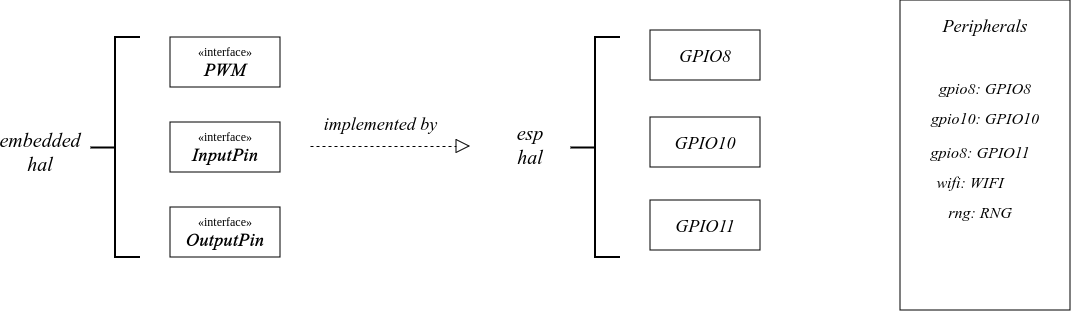
\includegraphics[scale=0.4]{images/rust/peripheral_pattern.drawio.png}
  \caption{HAL Pattern για τον ESP.}
  \label{fig:peripheral_pattern}
\end{figure}

Το \verb|Peripherals| struct υλοποιείται διαφορετικά ανάλογα με τον
μικροελεγκτή. Δηλαδή κάνουμε compile το esp-hal με ένα flag που
αντιπροσωπεύει το όνομα του MCU που χρησιμοποιούμε. Στo cargo, το αντίστοιχο
CMake της Rust, τα flags λέγονται features και γράφονται σε ένα αρχείο Cargo.toml
που βρίσκεται στο root του project:

\begin{lstlisting}
  [dependencies]
  ...other deps
  esp-hal = { version = "0.23.1", features = ["esp32c6", "unstable"] }
\end{lstlisting}

Η προσέγγιση του Peripheral ακολουθεί τις αρχές της
Rust που αναλύσαμε παραπάνω δηλαδή στο ότι κάθε περιφεριακό (USB
Port,GPIO-Pins,SPI,UART) αποτελεί έναν μοναδικό και καταναλώσιμο πόρο.
Κατά συνέπεια, μόλις το περιφερειακό ληφθεί από τη δομή που το
διαχειρίζεται (συνήθως μια δομή τύπου Peripherals), θεωρείται ότι
καταναλώθηκε και δεν μπορεί να χρησιμοποιηθεί ξανά χωρίς ρητή
επιστροφή του ελέγχου από το πρόγραμμα. Για παράδειγμα, ένα GPIO pin
(ψηφιακή θύρα εισόδου/εξόδου) μπορεί να χρησιμοποιηθεί είτε για είσοδο
είτε για έξοδο, αλλά ποτέ ταυτόχρονα, καθώς η πρώτη χρήση καταναλώνει
τον αντίστοιχο πόρο.



